\documentclass[9pt,aspectratio=43,mathserif,table]{beamer} 
%设置为 Beamer 文档类型,设置字体为 10pt,长宽比为16:9,数学字体为 serif 风格
\batchmode

% 加快编译, 发布时要改
%\includeonlyframes{current}
\includeonly{Tricks and Meaning}

\special{dvipdfmx:config z 0}
\usepackage{booktabs} % 表格上下粗线

\usepackage[backend=bibtex,sorting=none]{biblatex}
\setbeamerfont{footnote}{size=\tiny}
\addbibresource{ref_weekly.bib}
\usepackage[utf8]{inputenc}
\usepackage{graphicx}
\usepackage{animate}
\usepackage{hyperref}
\usepackage{diagbox} %表头斜线分区
\usepackage{makecell} %表头斜线分区
\usepackage{bbding} % 对错符号
%导入一些用到的宏包
\usepackage{xeCJK} %导入中文包
\setCJKmainfont{SimHei} %字体采用黑体  Microsoft YaHei
%\setmainfont{Times New Roman}
%\setmonofont{Courier New}
%\setCJKmainfont[AutoFakeBold = {2.15},ItalicFont={KaiTi}]{SimSun}
%\setCJKfamilyfont{xw}{STXinwei}
%%\setsansfont{Arial}
%\setsansfont{Microsoft YaHei}
\usepackage{unicode-math}
\usepackage{multicol}
\usepackage{amsmath,bm,amsfonts,amssymb,enumerate,epsfig,bbm,calc,color,ifthen,capt-of,multimedia,hyperref}
%\usepackage{bm, color}

\usepackage{newtxtext}
%\usepackage{newtxmath}

%\usepackage{tikz} % 圈中数字
%\usepackage{fontspec} % 圈中数字
%\usepackage{newtxtext}
%\usepackage[T1]{fontspec}
%更改样式
\renewcommand{\figurename}{Fig}
%\renewcommand*{\bibfont}{\footnotesize}

\usetheme{Berlin} %主题
\usecolortheme{sustech} %主题颜色

\usepackage[ruled,linesnumbered]{algorithm2e}

\usepackage{fancybox}
\usepackage{xcolor}
%\usepackage{times}
\usepackage{listings}

\usepackage{booktabs}
\usepackage{colortbl}

\newcommand{\Console}{Console}
\lstset{ %
	backgroundcolor=\color{white},   % choose the background color
	basicstyle=\footnotesize\rmfamily,     % size of fonts used for the code
	columns=fullflexible,
	breaklines=true,                 % automatic line breaking only at whitespace
	captionpos=b,                    % sets the caption-position to bottom
	tabsize=4,
	commentstyle=\color{mygreen},    % comment style
	escapeinside={\%*}{*)},          % if you want to add LaTeX within your code
	keywordstyle=\color{blue},       % keyword style
	stringstyle=\color{mymauve}\ttfamily,     % string literal style
	numbers=left, 
	%	frame=single,
	rulesepcolor=\color{red!20!green!20!blue!20},
	% identifierstyle=\color{red},
	language=c
}


\definecolor{mygreen}{rgb}{0,0.6,0}
\definecolor{mymauve}{rgb}{0.58,0,0.82}
\definecolor{mygray}{gray}{.9}
\definecolor{mypink}{rgb}{.99,.91,.95}
\definecolor{mycyan}{cmyk}{.3,0,0,0}

%题目,作者,学校,日期
\title{Nonlinear Dynamics and Chaos: With Apllications to Physics, Biology, Chemistry, and Engineering}
\subtitle{\fontsize{9pt}{14pt}\textbf{Weekly Reading Seminar}}
\author{Speaker: Xu Jie \quad \newline  \newline \quad Tutor: Zheng Zhigang}
\institute{\fontsize{8pt}{14pt}College of Information Science \& Engineering, Huaqiao University}
\date{\today}

%学校Logo
%\pgfdeclareimage[height=0.5cm]{sustech-logo}{sustech-logo.pdf}
%\logo{\pgfuseimage{sustech-logo}\hspace*{0.3cm}}

\AtBeginSection[]
{
	\begin{frame}<beamer>
	\frametitle{\textbf{Table of Contents}}
	\tableofcontents[currentsection]
\end{frame}
}
\beamerdefaultoverlayspecification{<+->}

\newcommand{\circlednumberone}{%
  \begin{tikzpicture}[baseline={(0,0)}, scale=0.8]
    \draw (0, 0) circle (1mm);
    \node at (0, 0) {1};
  \end{tikzpicture}%
}


% -----------------------------------------------------------------------------
\begin{document}
% -----------------------------------------------------------------------------

\frame{\titlepage}

\section[TOC]{}   %目录
\begin{frame}{TOC}
\tableofcontents
\end{frame}

% -----------------------------------------------------------------------------
\section{Start up}
\begin{frame}{Introduction}
  \begin{center}
   Hello, new comers

   \medskip

   Welcome to complex science! 

   \medskip

   Please Introduce yourself breifly.
  \end{center}

  \begin{itemize}
    \item [] 
    \item Chen Zhenyu
    \item Li Xinlong
    \item Liu Chang
    \item Lu Yichen
    \item Xu Yining
    \item Tian Zhuanghe
    \item Fan Weijun
    \item Introducing Our Group
  \end{itemize}

\end{frame}

\begin{frame}{What's nonlinear dynamics about}
    1. How do we represent research object?

    \bigskip

    The swinging of a pendulum

    $$\ddot x + \frac{ g}{L} \sin x = 0$$

    logistic model
    $$x_{n+1} = r x_n (1 - x_n)$$
\end{frame}

\begin{frame}{What's nonlinear dynamics about}
    2. What is nonlinearity

    The swinging of a pendulum,

    \bigskip

    $$\ddot x + \frac{ g}{L} \sin x = 0$$

    using ODE (ordinary differential equation) general framework, 
    \begin{equation}
      \begin{aligned}
        \dot x_1 &= f_1(x_1, \cdots, x_n)\\
        &\vdots \\
        \dot x_n &= f_1(x_1, \cdots, x_n)
      \end{aligned}
    \end{equation}
    coud be rewritten as

    \begin{equation}
      \begin{aligned}
        \dot x_1 &= x_2 \\
        \dot x_2 &= - \frac{ g}{L} \sin x_1
      \end{aligned}
    \end{equation}
\end{frame}
\begin{frame}{What's nonlinear dynamics about}
   In comparison, forced damping harmonic oscillator is governed by
   $$m \ddot x + b \dot x + kx  = 0$$

   using the ODE general framework, introducing new variables $x_1 = x, x_2=\dot x$, we can rewrite it to

    \begin{equation}
      \begin{aligned}
        \dot x_1 &= x_2 \\
        \dot x_2 &= - \frac{ b}{m}x_2 - \frac{ k}{m} x_1
      \end{aligned}
    \end{equation}

   which is called linear system.
\end{frame}
\begin{frame}{What's nonlinear dynamics about}
   If the force is time dependent F = F(t), say F(t) = $F\cos t$ (which is more general way), this type of system is called nonautonomous system.  

   the original ODE:

   $$m \ddot x + b \dot x + kx  = F\cos t$$

   We can still introducing new variable $x_3 = t$ and write the framework version:
    \begin{equation}
      \begin{aligned}
        \dot x_1 &= x_2 \\
        \dot x_2 &= - \frac{ b}{m}x_2 - \frac{ k}{m} x_1 + \frac{1}{m} F\cos x_3 \\
        \dot x_3 &= 1 
      \end{aligned}
    \end{equation}
\end{frame}
\begin{frame}{What's nonlinear dynamics about}
   3. How do we deal with nonlinear ODEs
    \begin{equation}
      \begin{aligned}
        \dot x_1 &= x_2 \\
        \dot x_2 &= - \frac{ g}{L} \sin x_1
      \end{aligned}
    \end{equation}

    3.1 figures 
    \begin{figure}[!h]
      \centering
      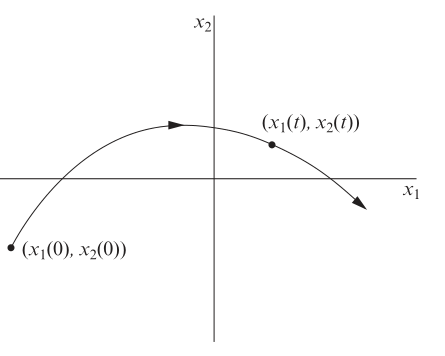
\includegraphics[width=.3\textwidth]{fig/trajectory.png}
      \caption{curve: trajectory}
    \end{figure}

    the space in the fig is called phase space, the number of variables $(x_1,x_2,\ldots,x_n)$ is called n-dimension or nth-order. This is an 2D or 2th-order system.

\end{frame}

\begin{frame}{How do we deal with nonlinear ODEs}
   3.2 numerical simulation

    \begin{figure}[!h]
      \centering
      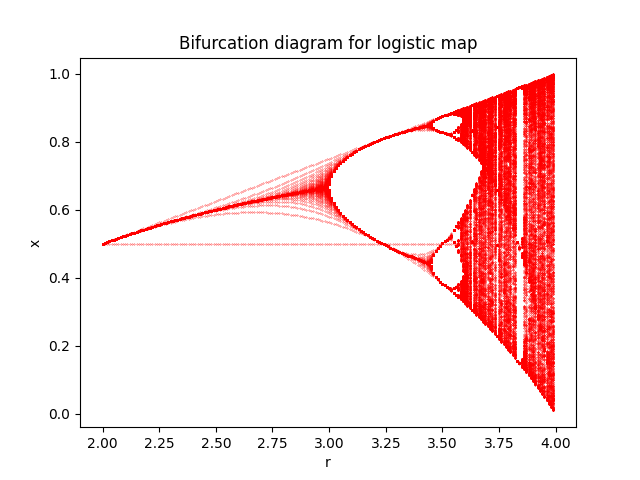
\includegraphics[width=.4\textwidth]{fig/logisticMap.png}
      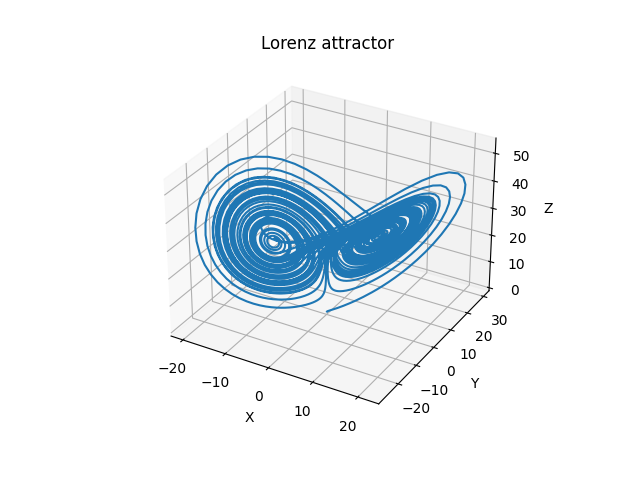
\includegraphics[width=.4\textwidth]{fig/Lorenz attractor.png}
      \caption{Logistic map(left) and Lorenz attractor(right)}
    \end{figure}


   3.3 linear stability analysis

   (referred later)

\end{frame}

\begin{frame}{Outline of this subject}
     \begin{figure}[!h]
      \centering
      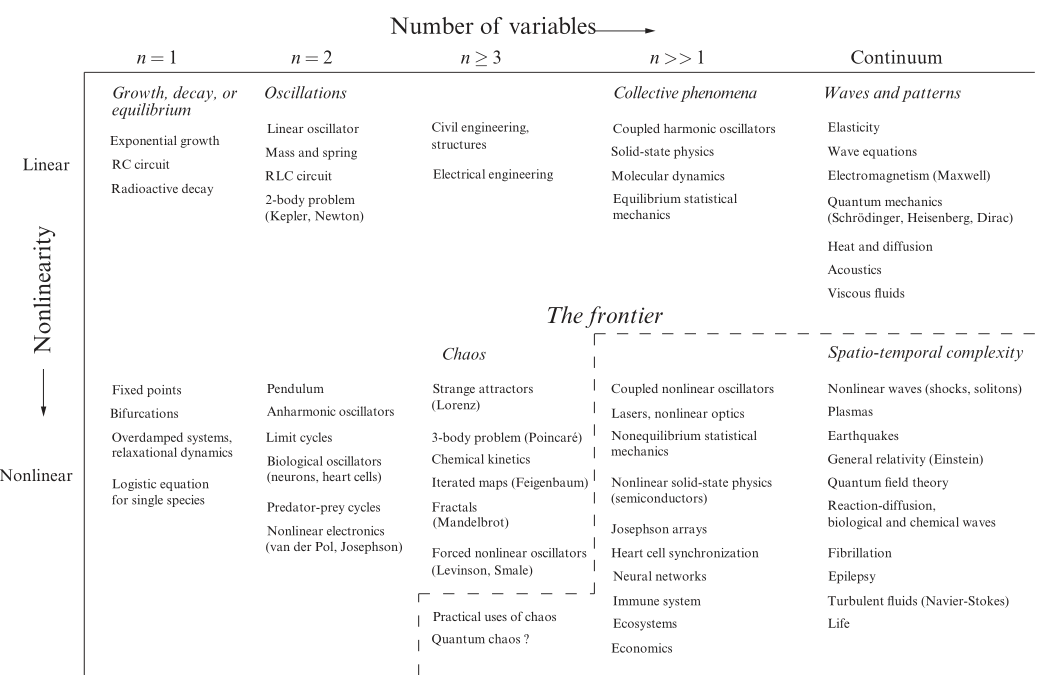
\includegraphics[width=.9\textwidth]{fig/problemMap.png}
      \caption{problem map}
    \end{figure}  
\end{frame}

\begin{frame}{History of this subject}
    \begin{figure}[!h]
      \centering
      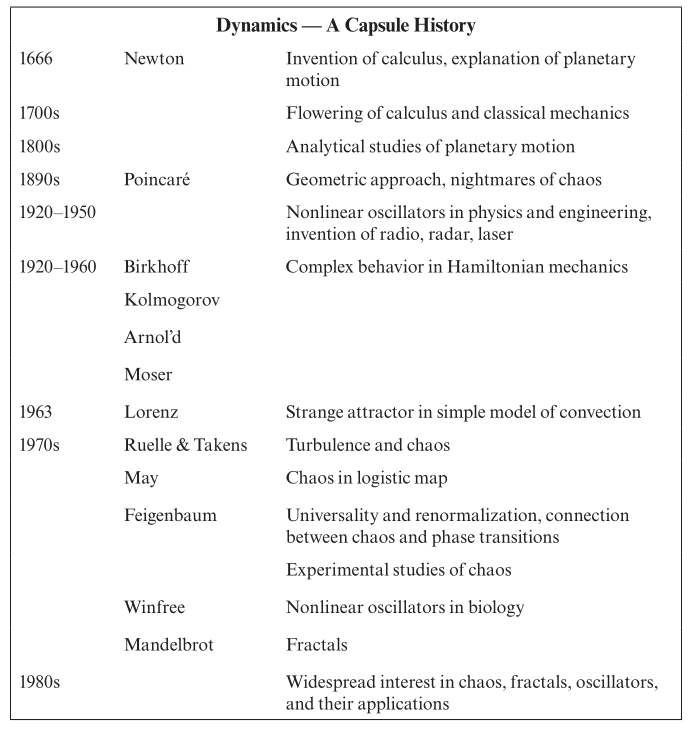
\includegraphics[width=.5\textwidth]{fig/history.png}
      \caption{history}
    \end{figure}
\end{frame}

\section{n=1 Intro.}
\begin{frame}{Let's get started!}
  \textcolor{red}{techneque: interpret ODE as a vecter field}
  \begin{multicols}{2}
  if n = 1, in the ODE framework, we obtain
  $\dot x = f(x)$
      consider this solvable ODE: 
      $$\dot x = \sin x$$

      or $\frac{ dx}{dt} = \sin x$

      seperate variables and then integrate

      $$dt = \frac{ dx}{\sin x}$$

      and obtain
          \begin{equation}
            \begin{aligned}
             t &= \int_{ }^{} \csc x dx \\
               &= - \ln |\csc x + \cot x| + C
            \end{aligned}
          \end{equation}

      To evaluate the constant C, suppose that  $x = x_0$at $t = 0$. Then $C = \ln | \csc x_0 + \cot x_0 |$. Hence the solution is
      $$t = \ln |\frac{ \csc x_0 + \cot x_0}{\csc x + \cot x}|$$

      the result is exact. But how about some questions:

      1. Suppose $x_0 = \frac{ \pi }{4}$; describe x(t), i.e. how the particle moves, particularly when $t \rightarrow \infty$

      2. For an arbitrary $x_0$, what's the behavior of x(t) as $t\rightarrow \infty$

  \end{multicols}
\end{frame}

\begin{frame}{vector field}
    
  \begin{multicols}{2}
    \begin{figure}[!h]
      \centering
      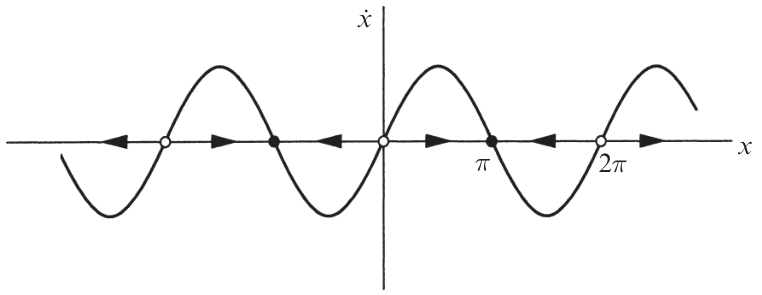
\includegraphics[width=.4\textwidth]{fig/vectorfield.png}
      \caption{2.1.1}
    \end{figure}

    Now we can answer these two question

      1. Suppose $x_0 = \frac{ \pi }{4}$; describe x(t), i.e. how the particle moves, particularly when $t \rightarrow \infty$

      2. For an arbitrary $x_0$, what's the behavior of x(t) as $t\rightarrow \infty$
    \begin{figure}[!h]
      \centering
      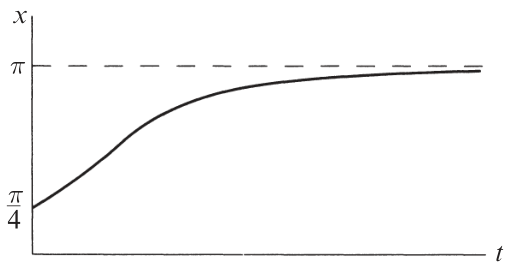
\includegraphics[width=.3\textwidth]{fig/solution_2.1.1.png}
    \end{figure}

       \begin{figure}[!h]
      \centering
      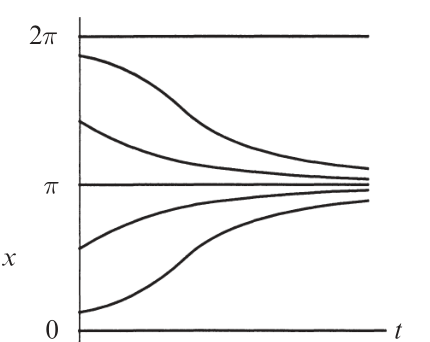
\includegraphics[width=.3\textwidth]{fig/solution_2.1.1_arbitraryinitial.png}
    \end{figure}
  \end{multicols}
\end{frame}

\begin{frame}{Glossory}
  \begin{multicols}{2}
   ODE

   nonautonomous

   linear system

   trajectory

   phase space

   logistic map

   Lorenz attractor

   linear stability analysis

   limit cycle 

   chaos

   fractals
   
   one-dimensional

   first order

  \end{multicols}
\end{frame}



\section{Tricks and Meaning}
\begin{frame}{What do we care about}
Stability

\bigskip

Stability under different condition 

\bigskip

behavior

\end{frame}

\begin{frame}{Is our focus valuable}
  \begin{multicols}{2}

  Example 
    2.3
    Logistic \textbf{Equations}

    $\dot N = r N (1 - \frac{ N}{K})$

    \begin{figure}[!h]
      \centering
      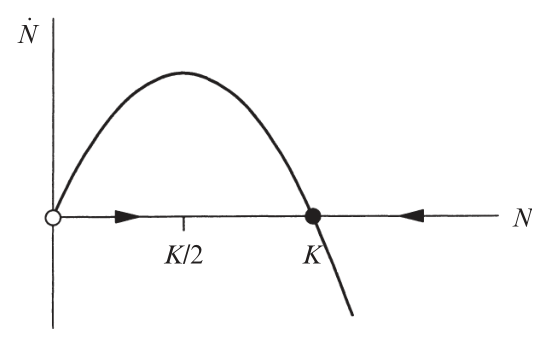
\includegraphics[width=.4\textwidth]{fig/logisticEq.png}
      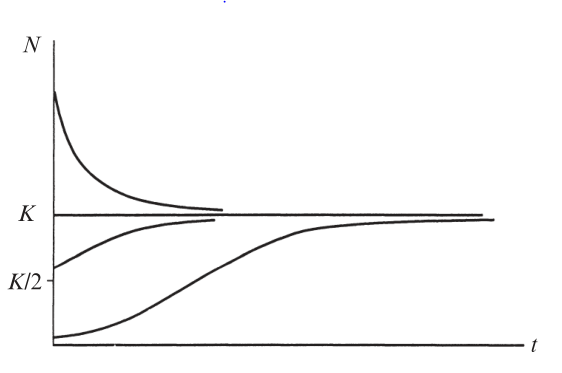
\includegraphics[width=.4\textwidth]{fig/logisticEq_xt.png}
    \end{figure}

  Exercise
    2.2.13
    An experimental study (Carlson et al. 1942) confirmed that the equation
    \textcolor{red}{$m\dot v = mg - kv^2$} gives a good quantitative fit to data on human skydivers

    2.3.3
    (Tumor growth) The growth of cancerous tumors can be modeled by the Gompertz law 
    \textcolor{red}{$\dot N = -a N \ln(bN)$}, where N (t) is proportional to the number of
    cells in the tumor, and a, b > 0 are parameters.

    The predictions of this simple model agree surprisingly well with data on tumor
    growth, as long as N is not too small; see Aroesty et al. (1973) and Newton (1980)
    for examples.


  \end{multicols}
   
  Phenomenon exists in ODEs models the reality!
\end{frame}

\begin{frame}{diverse dynamic behavior}
  basic magic

  Exercise

  2.4.9 Critical slowing down

  2.5.2 Blow up

\end{frame}

\begin{frame}{Uniqueness and Existance }  
  \begin{multicols}{2}
    Example 2.5.1 Show that the solution to  $$\dot x =  x ^ \frac{ 1}{3}$$ starting from $x_0 = 0$ is \textbf{not} unique.

    \medskip

    Solution: The point $x=0$ is a fixed point, so one obvious solution is $x (t) = 0$ for all t. 

    The surprising fact is that there is another solution. To find it we separate 
    variables and integrate:

    $$\int_{ }^{} x^{-\frac{ 1}{3}} dx = \int_{ }^{}dt $$

    So, $$\frac{ 3}{2} x ^{\frac{ 2}{3}} = t + C  $$ Imposing that $x_0 = 0$ yields $C=0$

    Hence  $$x(t) = (\frac{ 2}{3} t)^{\frac{ 3}{2}}$$ is also a solution

    In fact, there are infinitely many solutions (Exercise 2.5.4)
    \begin{figure}[!h]
      \centering
      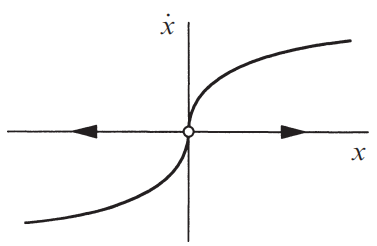
\includegraphics[width=.3\textwidth]{fig/uniqueness.png}
    \end{figure}
  \end{multicols}
  Theorem:  Consider the initial value problem 
  $x =  f (x), x (0) = x_0$, if $f(x), f'(x)$ are continuous on an open interval R, the problem has a unique solution x(t) on some time interval $(\tau, - \tau)$
\end{frame}

\begin{frame}{Uniqueness and Existance }
  \begin{multicols}{2}
   EXAMPLE 2.5.2: Discuss the existence and uniqueness of solutions to the initial value problem 
  $$\dot x = 1 + x^ 2 , x(0)= x_0.$$ Do solutions exist for all time?

  Solution: This right hand side is continuous and has a continuous derivatives, indicating existance at some interval, \textbf{not all the time}

  for example, consider $x(0) = 0$, by separation of variables:
  $$\int_{ }^{}\frac{ dx}{1 + x^2} = \int_{ }^{}dt$$

  which yields
  $$\arctan x = t + c$$

  Imposing $x(0) = 0$ yields $C = 0$. Hence  $$x(t) = \tan t$$ is the solution. But not that this solution exists only for $t \in (\frac{ -\pi}{2}, \frac{ \pi}{2})$

  \end{multicols}
  solution reaches infinity in finite time. This phenomenon is called \textbf{blow-up}.
\end{frame}

\begin{frame}{dominant of 1st-order systems}
    \begin{figure}[!h]
      \centering
      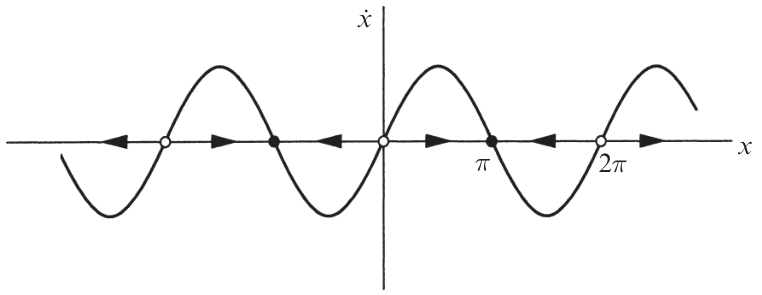
\includegraphics[width=.5\textwidth]{fig/vectorfield.png}
      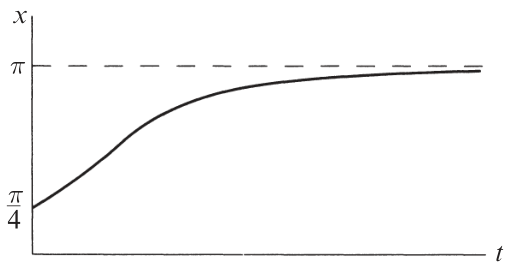
\includegraphics[width=.4\textwidth]{fig/solution_2.1.1.png}
    \end{figure}
all trajectories either approach a fixed point monotically, or diverged to $\pm \infty$

phase point never reverses direction.

\medskip

\textbf{Overshooting} is impossible.

\textbf{damped} oscillation is impossible

\textbf{undamped} oscillation is impossible (no periodic solutions)
   
\medskip 

explain this paradox (Exercise 2.6.1):
a simple harmonic oscillator $m\ddot x = -kx$ is a system that oscillates in one dimension (along the x-axis). But the text says one-dimensional systems can't oscillate.
\end{frame}




\begin{frame}{Another trick: Potential}
   Graph the potential for the system $\dot x = x - x ^ 3 $, and
   identify all equilibrium points.

    \begin{figure}[!h]
      \centering
      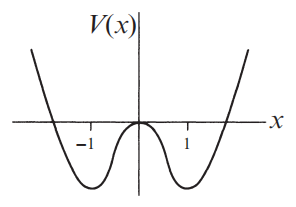
\includegraphics[width=.4\textwidth]{fig/bistable_potential.png}
      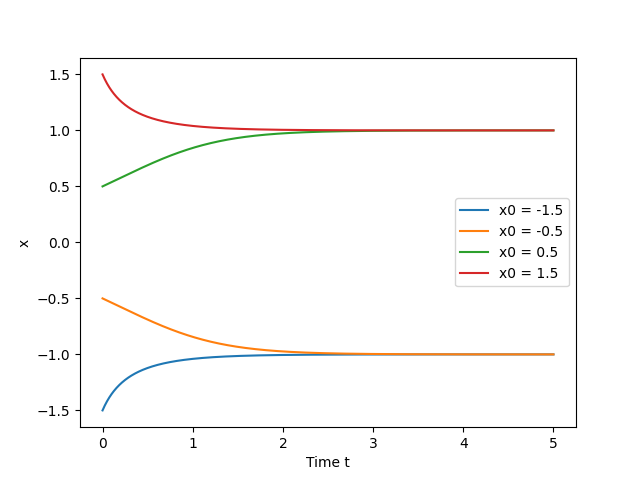
\includegraphics[width=.4\textwidth]{fig/bistable_solution.png}
    \end{figure}

\end{frame}

\begin{frame}{Summerize tricks}
    \begin{figure}[!h]
      \centering
      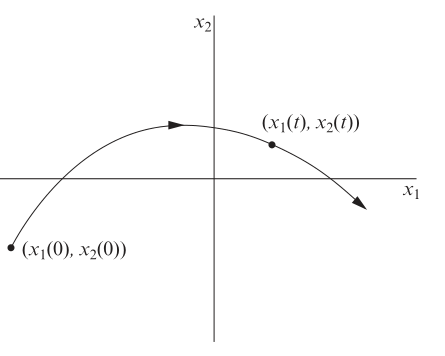
\includegraphics[width=.3\textwidth]{fig/trajectory.png}
      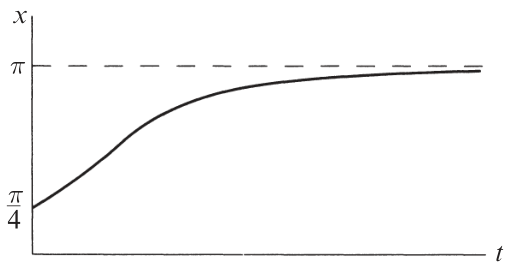
\includegraphics[width=.3\textwidth]{fig/solution_2.1.1.png}
      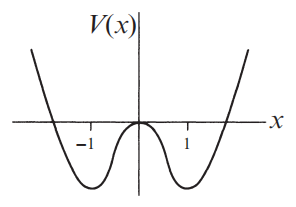
\includegraphics[width=.3\textwidth]{fig/bistable_potential.png}
      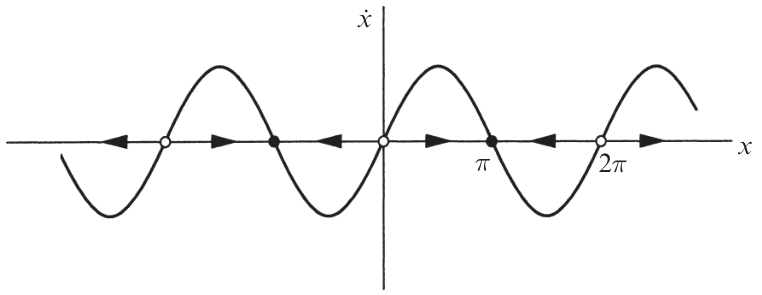
\includegraphics[width=.3\textwidth]{fig/vectorfield.png}
      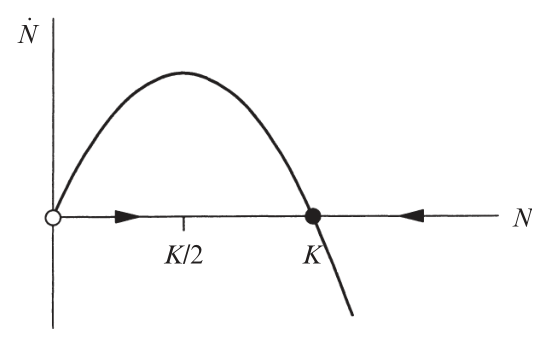
\includegraphics[width=.3\textwidth]{fig/logisticEq.png}
      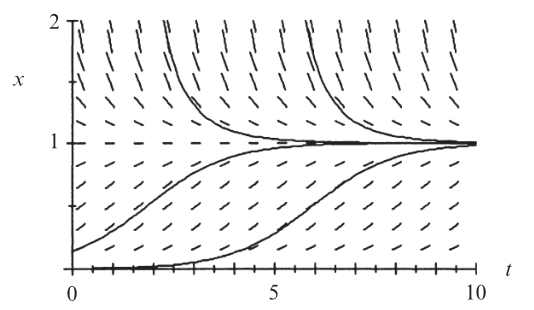
\includegraphics[width=.3\textwidth]{fig/slopefield.png}
    \end{figure}
   
\end{frame}



\begin{frame}{Bifuractions}
   Saddle-Node  $\dot x = r + x^2$

   Transcritical $\dot x = rx - x^2$

   \medskip

   Pitchfork 
     
     Supercritical Pitchfork  $\dot x = rx - x ^3$

     Subcritical Pitchfork $\dot x = rx + x^3 - x^5$

   Imperfect Bifurcations and Catastrophes  $\dot x = h + rx - x^3$
\end{frame}

\begin{frame}{Saddle node}
   $\dot x = r + x^2$
    \begin{figure}[!h]
      \centering
      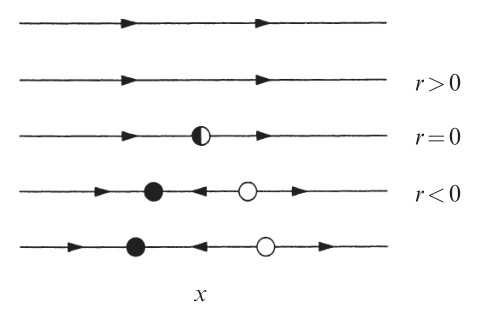
\includegraphics[width=.4\textwidth]{fig/saddelnode_vectorfield.PNG}
      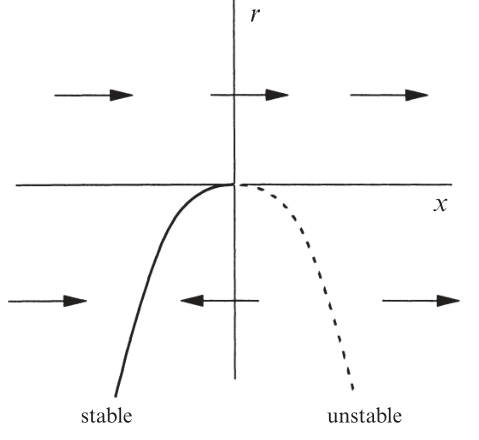
\includegraphics[width=.4\textwidth]{fig/saddelnode_vectorfield_continuousstack.PNG}
    \end{figure}
    \begin{figure}[!h]
      \centering
      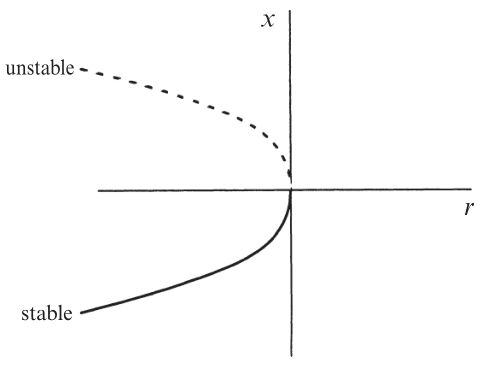
\includegraphics[width=.3\textwidth]{fig/saddelnode_vectorfield_continuousstack_invertaxes.png}
    \end{figure}
\end{frame}
\begin{frame}{Transcritical}
    $\dot x = rx - x^2$
    \begin{figure}[!h]
      \centering
      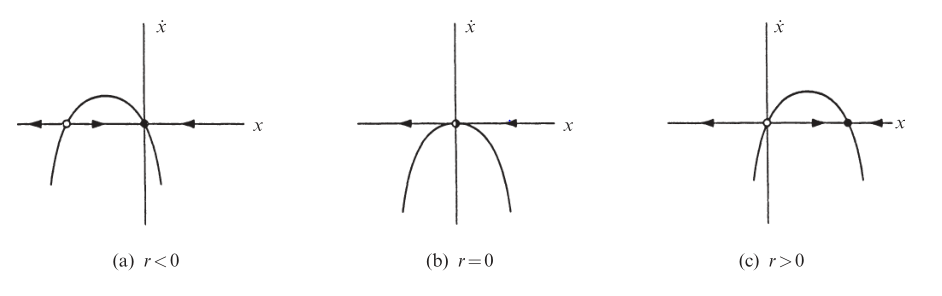
\includegraphics[width=.8\textwidth]{fig/transcritical.png}
      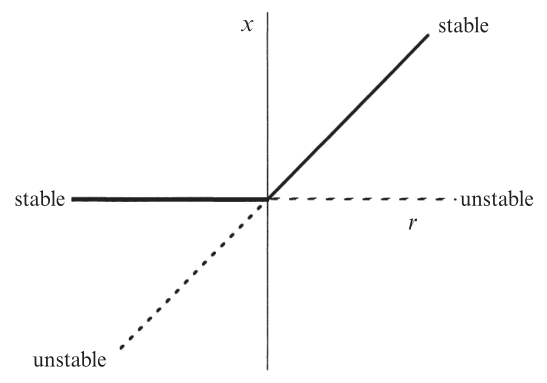
\includegraphics[width=.4\textwidth]{fig/transcritical_bifurcation.png}
    \end{figure}
\end{frame}
\begin{frame}{Pitchfork: Supercritical}
    $\dot x = rx - x ^3$
     \begin{figure}[!h]
      \centering
      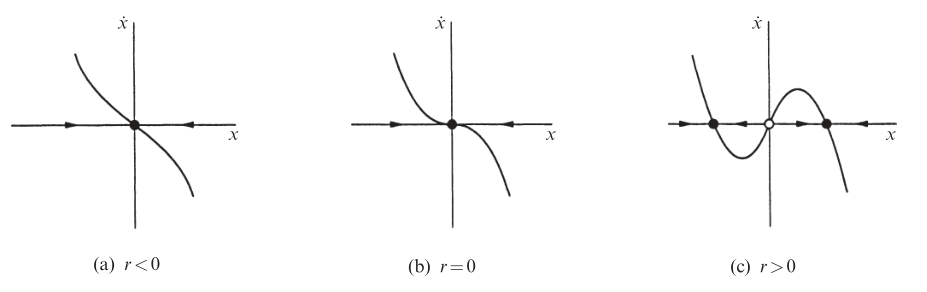
\includegraphics[width=.8\textwidth]{fig/supercriticalPitchfork.PNG}
      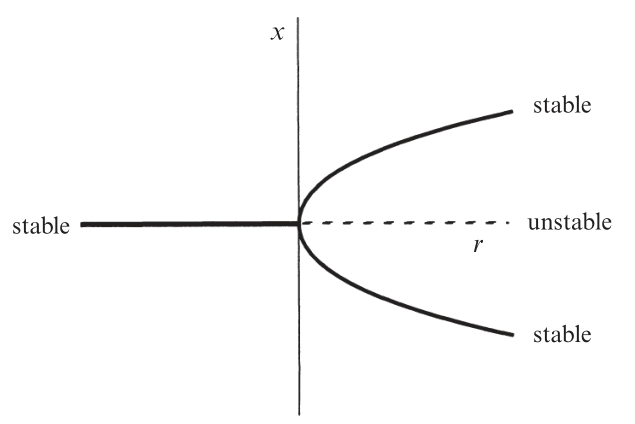
\includegraphics[width=.4\textwidth]{fig/supercriticalPitchfork_bifurcation.PNG}
      \caption{}
    \end{figure}
 
\end{frame}
\begin{frame}{Pitchfork: Subcritical}
     Subcritical Pitchfork $\dot x = rx + x^3 - x^5$
   
    \begin{figure}[!h]
      \centering
      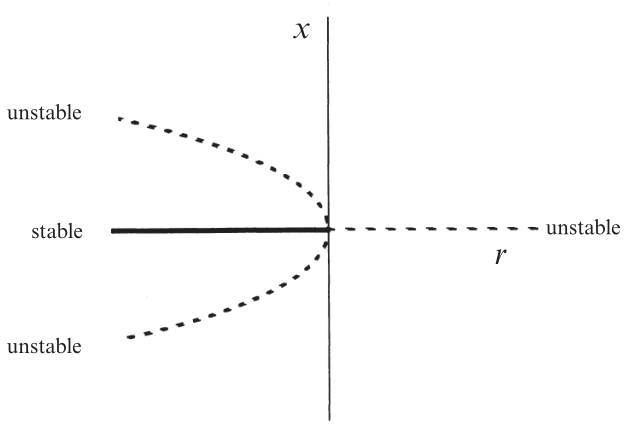
\includegraphics[width=.5\textwidth]{fig/subcritical_bifurcation_unstable.png}
      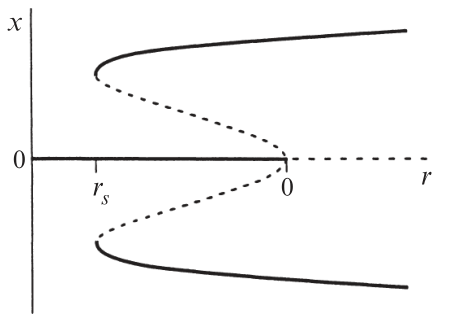
\includegraphics[width=.4\textwidth]{fig/subcritical_bifurcation.png}
    \end{figure}
 
\end{frame}
\begin{frame}{Glossary}
  undamped

  underdammped

  overdamped

  Transcritical

  Supercritical

  Subcritical
   
\end{frame}


\section{Bifurcation}
\begin{frame}{Trick: drawing a bifurcation diagram}
   
  \begin{multicols}{2}
   Example 3.4.1

   $\dot x = - x + \beta \tanh x$

    \begin{figure}[!h]
      \centering
      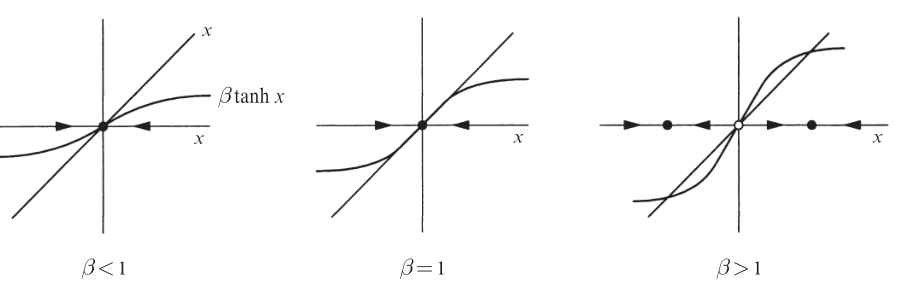
\includegraphics[width=.5\textwidth]{fig/betatanhx.png}
    \end{figure}
 
   One way is to find roots of the equation, for EACH $\beta$

   Another way is calculating

   $\beta = \frac{ x}{ \tanh x}$

   for a set of x values, and obtain (beta, x) for plotting

    \begin{figure}[!h]
      \centering
      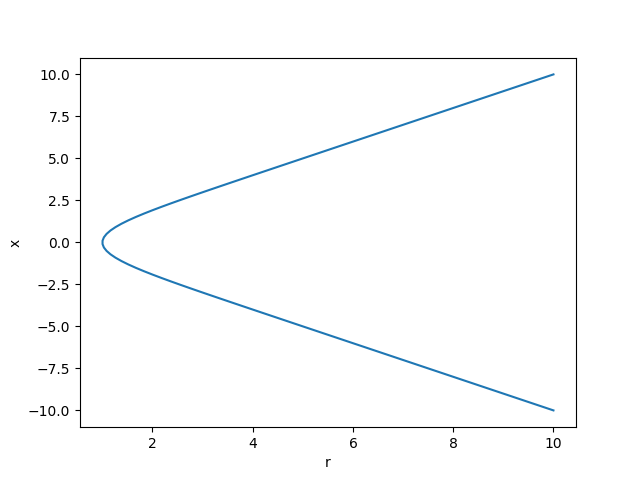
\includegraphics[width=.5\textwidth]{fig/betatanhx_bifurcation.png}
    \end{figure}
 
  WARNING: stability analysis required!
  \end{multicols}

\end{frame}
\begin{frame}{Saddle Node}

  \begin{multicols}{2}
   standard form  $\dot x = r + x^2$

   \medskip

   form $\dot x = r -  x - e^{-x}$ (example 3.1.2)

   \medskip

   exercise 3.1.1 - 3.1.4

   $\dot x = 1 + rx + x^2$

   $\dot x = r - \cosh x$

   $\dot x = r + x - \ln(1+x)$

   $\dot x = r + \frac{ 1}{2}x - \frac{ x}{1+x}$

    \begin{figure}[!h]
      \centering
      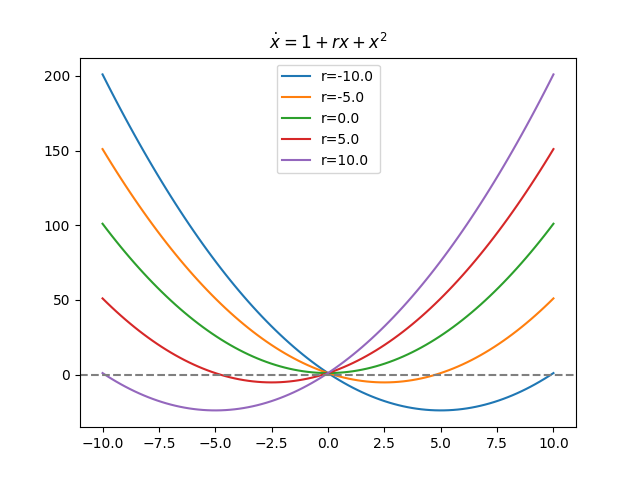
\includegraphics[width=.3\textwidth]{fig/saddlenode-1.png}
      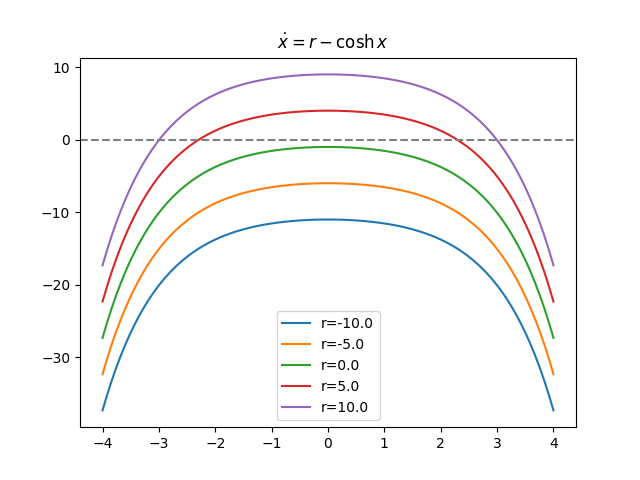
\includegraphics[width=.3\textwidth]{fig/saddlenode-2.png}
    \end{figure}
 
   \end{multicols}

   Question: How can we tell if a bifurcation is Saddle-Node type?
   
\end{frame}

\begin{frame} {Transcritical}
  \begin{multicols}{2}
   standard form  $\dot x = rx - x^2$

   \medskip

   form $x(1-x^2) - a(1-e^{-bx})$ (example 3.1.2)

   \medskip

   exercise 3.1.1 - 3.1.4

   $\dot x = r x + x ^ 2$

   $\dot x = r  x - \ln(1+x)$

   $\dot x = x - r  x  (1-x)$

   $\dot x = x  (r - \exp(x))$

    \begin{figure}[!h]
      \centering
      \includegraphics[width=.5\textwidth]{fig/transcritical-1.png}
    \end{figure}
 
   \end{multicols}

\end{frame}
\begin{frame}{An Example of Transcritical: laser model}

  \begin{multicols}{2}
    \begin{equation}
      \begin{aligned}
        \dot n &= gain - loss \\
               &= GnN - kn 
      \end{aligned}
    \end{equation}
    The dynamical variable is the number of photons $n ( t )$ in the laser field

    G, k is constant

    $N(t)$ denotes the rate of random encounter of photon and exited atoms

    the key physical idea: after an excited atom emits a photon, it
    drops down to a lower energy level and is no longer excited. 

    $$N(t) = N_0 - \alpha n$$

    Finnally 

    \begin{equation}
      \begin{aligned}
        \dot n &= Gn(N_0 - \alpha n) - k n \\
               &= (GN_0 - k) n - (\alpha G) n^2
      \end{aligned}
    \end{equation}

  \end{multicols}
    \begin{figure}[!h]
      \centering
      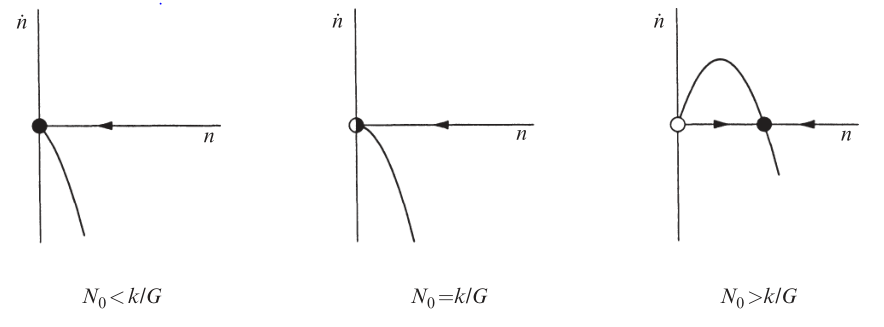
\includegraphics[width=.4\textwidth]{fig/laser_transcritical.png}
      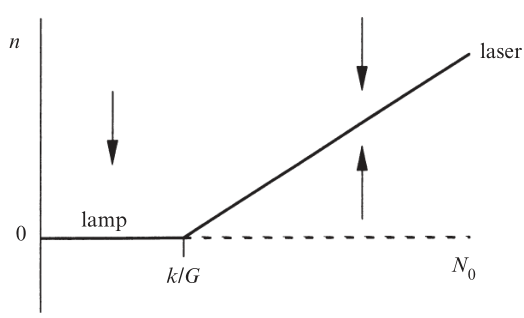
\includegraphics[width=.2\textwidth]{fig/laser_transcritical_bifurcation.png}
    \end{figure}
 
\end{frame}
\begin{frame}{Imporved Laser model}

  \begin{multicols}{2}
exercise 3.3.1 
In realistic way, the idea that N(t) is proportional to n would be replaced by a differential equation. For instance, Milonni and Eberly (1988) show that after certain reasonable approximations, quantum mechanics leads to the system
    \begin{equation}
      \begin{aligned}
        \dot n &= GnN - k n \\
        \dot N &= -GnN - f N + p
      \end{aligned}
    \end{equation}

    This two-dimensional system will be analyzed in Exercise 8.1.13. For now, let's convert it to a one-dimensional system, as follows.

    Suppose that N relaxes much more rapidly than n. Then we may make the quasi-static approximation $\dot N \approx 0$ (This procedure is often called \textbf{adiabatic elimination}, and one says that the evolution of $N ( t )$ is slaved to that of $ n ( t )$

    Thus obtaining $$N = \frac{p}{Gn + f}$$

    substituting N in $\dot n$, writes
    $$\dot n  = \frac{ Gnp}{Gn + f}- kn$$
  \end{multicols}
\end{frame}


\begin{frame}{Pitchfork}

  \begin{multicols}{2}
  standard form:

  \quad Supercritical Pitchfork  $\dot x = rx - x ^3$

  \quad Subcritical Pitchfork $\dot x = rx + x^3 - x^5$

  other forms (exercise 3.4.1 - 3.4.4)

   $$ \dot x = rx + 4 x ^ 3 $$
   $$ \dot x = rx - \sinh(x) $$
   $$ \dot x = rx - 4 x ^ 3 $$
   $$ \dot x = x / ( 1 + x ^ 2 ) $$

    \begin{figure}[!h]
      \centering
      \includegraphics[width=.5\textwidth]{fig/pitchfork.png}
      \includegraphics[width=.5\textwidth]{fig/pitchfork_potential.png}
      \caption{}
    \end{figure}
 
  \end{multicols}
\end{frame}
\begin{frame}{Glossary}
Adiabatic elimination

Critical damping

Critical slowing down


\end{frame}




\section{Models}


\begin{frame}{Critical Damping}

  $$\ddot x + \gamma\dot x + \omega^2 x = 0$$
  \begin{multicols}{2}
    $x(t) = e ^{-st}$

    $\Rightarrow (s^2 - \gamma s + \omega ^2)e^{st} = 0$

    $\Rightarrow s = -\frac{ 1}{2} (\gamma \pm \sqrt{\gamma^2 - 4 \omega ^2})$

    \bigskip

    Critical damping

    $\sqrt{\gamma^2 - 4 \omega ^2} = 0$

    $\gamma_c = 2 \omega $

    \bigskip

    When $\gamma = 0$ 

    $x(t) = e^{st} = e^{\pm i\omega t}$

    \medskip

    When $\gamma < \gamma_c$ 

    $x(t) = e^{st} = e^{-\frac{ 1}{2}\gamma C t}e^{\pm i\omega t}$

    \medskip

    When $\gamma = \gamma_c$ 

    $x(t) = e^{st} = e^{-\frac{ 1}{2}\gamma t} = e^{-\omega t}$

    characteristic time scale: $t = \frac{ 1}{\omega }$

  \end{multicols}
\end{frame}

\begin{frame}{Overdamped Bead on a Rotating Hoop}

  \begin{multicols}{2}
    \begin{figure}[!h]
      \centering
      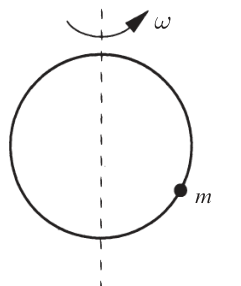
\includegraphics[width=.12\textwidth]{fig/overdamped1.png}
      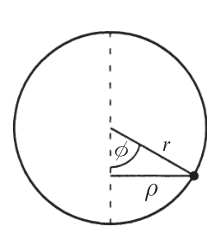
\includegraphics[width=.12\textwidth]{fig/overdamped2.png}
      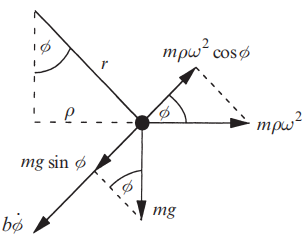
\includegraphics[width=.12\textwidth]{fig/forceanalysis.png}

    \end{figure}

    $$m r \ddot\phi = - b \dot \phi - mg \sin \phi + m r \omega ^2 \sin\phi\cos\phi$$

    throwing second-order term, obtain


    \begin{equation}
      \begin{aligned}
        b \dot \phi &= - mg \sin \phi + m r \omega ^2 \sin\phi\cos\phi \\
                    &= mg\sin\phi(\frac{ r\omega ^2}{g}\cos\phi - 1)
      \end{aligned}
    \end{equation}

    $\gamma = \frac{ r \omega ^ 2}{g}$, when $\gamma \gg 1$, $\phi \rightarrow \pm \frac{ \pi}{2}$

    \begin{figure}[!h]
      \centering
      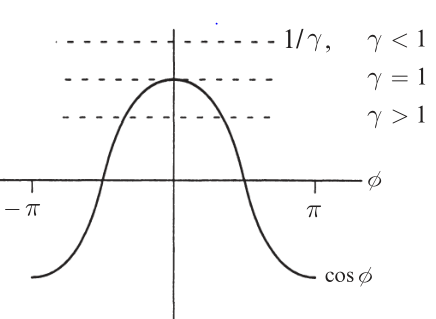
\includegraphics[width=.3\textwidth]{fig/overdamped-gamma.PNG}
      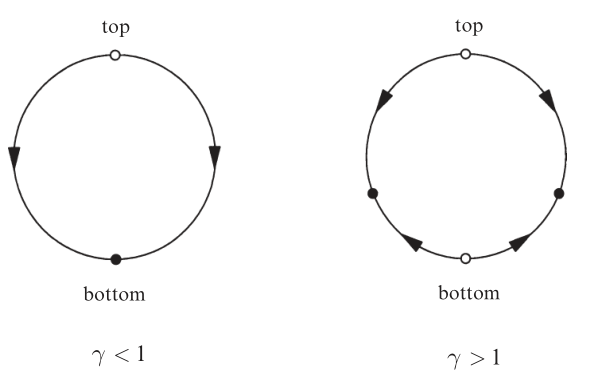
\includegraphics[width=.3\textwidth]{fig/overdamped-gamma2.PNG}
      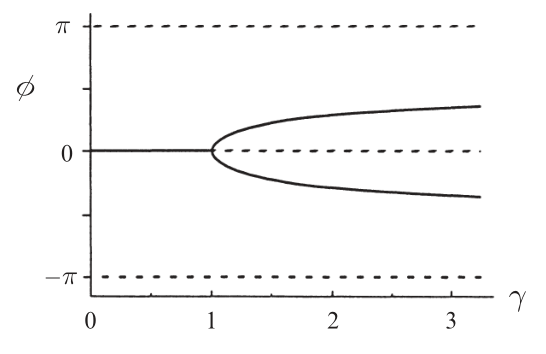
\includegraphics[width=.3\textwidth]{fig/overdamped-gamma-bifur.PNG}
    \end{figure}
 
  \end{multicols}
 
\end{frame}

\begin{frame}{Dimensional Analysis and Scaling}

    $$m r \ddot\phi = - b \dot \phi - mg \sin \phi + m r \omega ^2 \sin\phi\cos\phi$$

    $\tau = \frac{ t}{T}$

    $\dot \phi = \frac{ d\phi}{dt} = \frac{ d\phi}{d\tau}\frac{ d\tau}{dt} = \frac{ 1}{T} \frac{ d\phi}{d\tau}$
    \quad\quad $\ddot \phi =  \frac{ 1}{T^2} \frac{ d^2\phi}{d\tau^2}$

    $\frac{ mr}{T^2} \frac{ d^2\phi}{d\tau^2} = - \frac{ b}{T}\frac{ d\phi}{d\tau}  - mg\sin\phi + mr\omega ^2 \sin\phi + mr\omega ^2\sin\phi\cos\phi$

    $$(\frac{ r}{gT^2})\frac{ d^2\phi}{d\tau^2} = - (\frac{ b}{mgT}\frac{ d\phi}{d\tau}) - \sin\phi+(\frac{ r\omega ^2}{g})\sin\phi\cos\phi$$

    %①②③④⑤⑥⑦⑧⑨⑩
    we need $\frac{ r}{gT^2} \ll 1$ \symbol{2460} and $\frac{ b}{mgT}\approx \mathcal{O}(1)$②

    natural choice derived from ②

    $T = \frac{ b}{mg}$

    leading condition $\frac{ r}{ gT^2}\ll 1$ becomes

    $\frac{ r}{g} (\frac{ mg}{b})^2 \ll 1$
    or equivalently,
    $b^2 \gg m^2gr$

    interpreted as saying that damping is very strong


    introduce $\epsilon = \frac{ m^2 g r}{b^2}$

    $$\epsilon \frac{ d^2\phi}{d\tau^2} = - \frac{ d\phi}{dt} - \sin\phi + \gamma\sin\phi\cos\phi$$

\end{frame}
\begin{frame}{Dimensional Analysis}
\textbf{Buckingham $\pi$ theorem}
 
 $n$ variables can be equivalently rewritten as an equation of $n - m$ dimensionless parameters

 $$F - \mu mg = m a$$

 5 variables involves dimension (L,M,T), according to $\pi$ theorem, this eq can be rewritten using 2 dimensionless variables 
 $$\frac{ F}{ma} - \frac{ \mu mg}{ma} = 1$$

 generally, using SI standard, dimension of quantity Q can be written in the following format

 $$\dim Q = T^{a}L^{b}M^cI^d\Theta^eN^fJ^g$$

\end{frame}

\begin{frame}{Overdamped Pendulum}

  \begin{multicols}{2}
    \begin{figure}[!h]
      \centering
      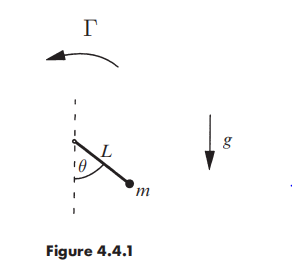
\includegraphics[width=.2\textwidth]{fig/4.4.1.png}
    \end{figure}
    The Newton's law yields
    $$m L^2 \ddot \theta + b \dot\theta + mgL\sin\theta = \Gamma$$

    neglecting $\ddot\theta$

    $$b\dot \theta+ mgL\sin\theta = \gamma$$

    nondimensionalize, 

    $$\frac{ b}{mgL}\dot\theta = \frac{ \Gamma}{mgL} - \sin\theta$$

    and finally 

    $$\theta' = \gamma - \sin\theta$$

    where $\theta' = \frac{ d\theta}{d\tau}$
  \end{multicols}
 
\end{frame}
\begin{frame}{Superconducting Josephson Junction}
    \begin{figure}[!h]
      \centering
      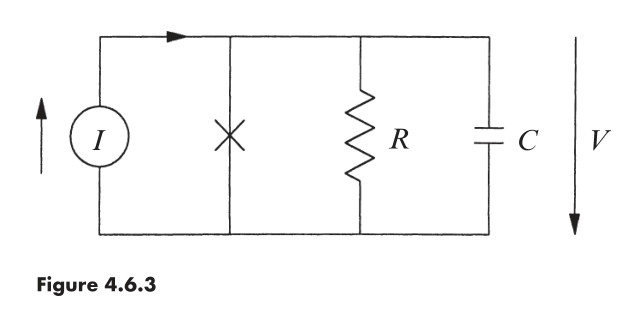
\includegraphics[width=.5\textwidth]{fig/Josephson Junction}
    \end{figure}
 
$$C\dot V + \frac{ V}{R} + I_c\sin\phi = I$$

$$\frac{ hC}{2e} \ddot \phi+ \frac{ h}{2eR}\dot\phi + I_c\sin\phi = I$$

is just like 

$mL^2 \ddot \theta + b\dot\theta + mgL\sin\theta = \Gamma$

\end{frame}




\begin{frame}{Time scale and adiabatic elimination}
  $$\epsilon \ddot x + \dot x + x = 0$$


  \begin{multicols}{2}
    $x(t) = e^{st}$

    $(s^2 \epsilon + s + 1)e^{st} = 0$

    $s = \frac{ 1}{2\epsilon}( -1 \pm \sqrt{1 - 4 \epsilon })$

    when $\epsilon \ll 1$, $s \rightarrow -\frac{ 1}{\epsilon}, -1$

    solution $e^{st} \rightarrow e^{-t}, e^{-\frac{ 1}{\epsilon} t} $
    
    Thus we obtain general solution 

    $$x(t) = C_1 e^{-t} + C_2e^{-\frac{ 1}{\epsilon}t}$$

    \medskip

    when $\epsilon \ll 1$ 

    $C_2$ term converge to 0 very fast, if $C_2$ isn't very different from $C_1$. and thus 
    $$x(t) \approx C_1 e^{-t}$$

    \begin{figure}[!h]
      \centering
      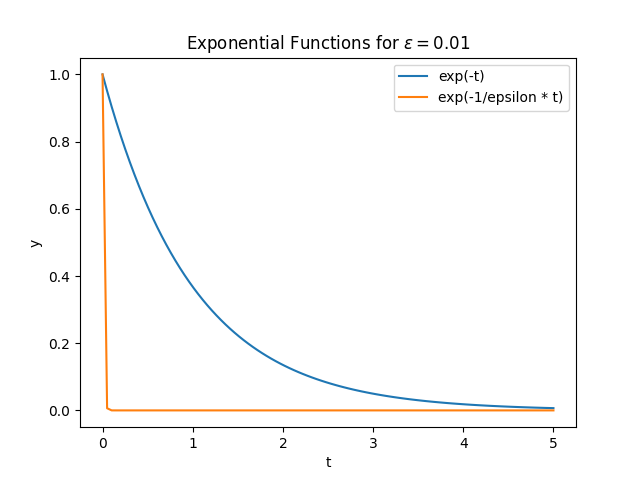
\includegraphics[width=.5\textwidth]{fig/3.5.6epsilon.png}
    \end{figure}
 
  \end{multicols}
\end{frame}


\begin{frame}{ Ising model}
$$\displaystyle  m = |\frac{ 1}{N} \sum_{i=1}^N S_i |$$
   $$h = T \tanh^{-1}m - J n m$$
\end{frame}

\begin{frame}{Glossary}

  \begin{multicols}{2}
    Dimensional analysis
    \\ dimensionless groups
    \\ nondimensionalize
    \\ transient
    \\ singular limit
    \\ pattern

    \medskip
   
    phase
    \\ phase difference
    \\ beat phenomenon
    \\ entrained
    \\ phase drift
    \\ resetting strength
    \\ phase-locked
    \\ range of entrainment
  \end{multicols}

\end{frame}


\section{2D}
\begin{frame}{2D linear system}

  \begin{multicols}{2}
    \begin{equation}
      \begin{aligned}
        \dot x &= a x + b y \\
        \dot y &= c x + d y
      \end{aligned}
    \end{equation}

    $\dot \mathbf{x} = A\mathbf{x}$

    where
    \begin{equation}
      \begin{aligned}
        A = 
        \begin{pmatrix}
          a & b \\
          c & d 
        \end{pmatrix}
      \end{aligned}
    \end{equation}

    Example  5.1.1 
    $$m \ddot x + k x = 0$$

    \begin{figure}[!h]
      \centering
      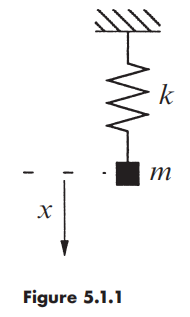
\includegraphics[width=.2\textwidth]{fig/5.1.1.sho.png}
    \end{figure}

    setting $\omega ^2 = \frac{ k}{m}$
    \begin{equation}
      \begin{aligned}
        \dot x &= v \\
        \dot v &= - \omega^2 x
      \end{aligned}
    \end{equation}

  \end{multicols}
\end{frame}

\begin{frame}{2D system vector field}
  \begin{multicols}{2}
    \begin{figure}[!h]
      \centering
      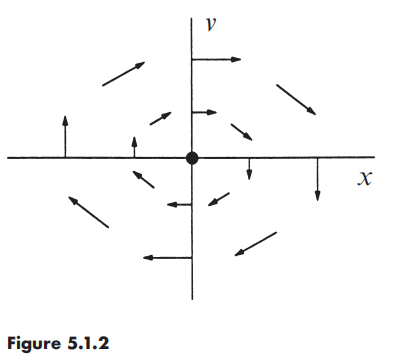
\includegraphics[width=.3\textwidth]{fig/5.1.2 vecterfield.png}
      \includegraphics[width=.3\textwidth]{fig/5.1.3 phaseportrait.png}
      \includegraphics[width=.4\textwidth]{fig/5.1.4 phase chart.png}
    \end{figure}

    vector field

    fixed point

    phase point

    phase portrait

    closed orbits

  \end{multicols}
\end{frame}
\begin{frame}{2D system with parameter }

  \begin{multicols}{2}
    Example 5.1.2 

    Solve the linear system $\dot \mathbf{x} = A \mathbf{x}$, where $A =  (\begin{smallmatrix} a & 0 \\ 0 & -1 \end{smallmatrix})$ Graph the phase portrait as a varies from $-\infty$ to $+\infty$, showing the qualitatively different cases.
    \small{
    \begin{equation}
      \begin{aligned}
        \begin{pmatrix}
          \dot x \\
          \dot y 
        \end{pmatrix}
         = 
        \begin{pmatrix}
          a & 0 \\
          0 & -1 
        \end{pmatrix}
        \begin{pmatrix}
          x \\
          y 
        \end{pmatrix}
      \end{aligned}
    \end{equation}
    }
    
    \begin{equation}
      \begin{aligned}
        \dot x &= ax \\
        \dot y &= -y 
      \end{aligned}
    \end{equation}
    un coupled eq, has solution

    \begin{equation}
      \begin{aligned}
         x(t) &= x_0 e^{at}\\
         y(t) &= y_0 e^{-t}
      \end{aligned}
    \end{equation}


    stable node 

    star

    saddle point
    \begin{figure}[!h]
      \centering
      \includegraphics[width=.5\textwidth]{fig/5.1.5phase diagram.png}
    \end{figure}
    stable manifold 

    unstable manifold
 \end{multicols}
 attracting;  globally attracting; 
 Liapunov stable;  neutrally stable
\end{frame}
\begin{frame}{2D system with general parameter}
  \begin{multicols}{2}

    \begin{equation*}
      \begin{aligned}
      \symbf{A} = 
        \begin{pmatrix}
          a & b \\
          c & d
        \end{pmatrix}
      \end{aligned}
    \end{equation*}

    we have explorerd

    \begin{equation*}
      \begin{aligned}
      \symbf{A} = 
        \begin{pmatrix}
          a & 0 \\
          0 & -1
        \end{pmatrix}
      \end{aligned}
    \end{equation*}

    and

    \begin{equation*}
      \begin{aligned}
      \symbf{A} = 
        \begin{pmatrix}
          0 & 1 \\
          -\omega^2  & 0
        \end{pmatrix}
      \end{aligned}
    \end{equation*}




    finding \textbf{straight-line trajectories} $\symbf{x}(t) = e^{\lambda t}\symbf{\symbf{v}}$

    for $\symbf{\dot {x}} =  \symbf{Ax}$

    and obtain

    $\symbf{Av}= \lambda \symbf{v}$

    this conclude that straight-line trajectories is an \textbf{eigenvector}

    For a 2$\times$2 matrix, the characteristic equation becomes


    \begin{equation*}
      \begin{aligned}
        det
        \begin{pmatrix}
          a-\lambda & b\\
          c & d-\lambda
        \end{pmatrix}
         = 0
      \end{aligned}
    \end{equation*}

    expanding the determinant yields

    \begin{equation}
      \begin{aligned}
        \lambda^2 - \tau\lambda + \delta = 0
      \end{aligned}
    \end{equation}

    where 
    $\tau = trace(A) = a + d$
    $\delta = det(A) = ad - bc$

    then
    $\lambda_1 = \frac{ 1}{2} (\tau + \sqrt{\tau ^2 - 4\delta})$,
    $\lambda_2 = \frac{ 1}{2} (\tau - \sqrt{\tau ^2 - 4\delta})$
    
    are the solutions of the quadratic equation
    
  \end{multicols}
\end{frame}
\begin{frame}{2D system with general parameter}

  \begin{multicols}{2}
 Example 5.2.1
  Solve the initial value problem $\dot x = x + y$, $\dot y = 4x-  2y$ , subject to the initial condition $( x_0 , y_0) = (2, -3)$.

  \medskip

  Solution:

    \begin{equation*}
      \begin{aligned}
      \symbf{A} = 
        \begin{pmatrix}
          1 & 1 \\
          4 & -2
        \end{pmatrix}
      \end{aligned}
    \end{equation*}

   has $\tau = -1$ and $\delta = -6$, the characteristic equation is $\lambda ^2 + \lambda - 6$, Hence
   $$\lambda_1 = 2, \lambda_2 = -3$$. Next, solving
   
    \begin{equation}
      \begin{aligned}
        \begin{pmatrix}
          1-\lambda & 1 \\
          4 & -2-\lambda
        \end{pmatrix}
        \begin{bmatrix}
          v_1\\
          v_2
        \end{bmatrix}
        =
        \begin{pmatrix}
          0\\
          0
        \end{pmatrix}
      \end{aligned}
    \end{equation}
    
    and obtain

    \begin{equation*}
      \begin{aligned}
        \symbf{v}_1 = 
        \begin{bmatrix}
          1\\
          1
        \end{bmatrix}
      \end{aligned}
      ,
        \symbf{v}_2 = 
        \begin{bmatrix}
          1\\
          -4
        \end{bmatrix}
    \end{equation*}
    the general solution is 
    \begin{equation*}
      \begin{aligned}
        \symbf{x}(t) = c_1
        \begin{bmatrix}
          1\\
          1
        \end{bmatrix}
        e^{2t}
        + c_2
        \begin{bmatrix}
          1\\
          -4
        \end{bmatrix}
        e^{-3t}
      \end{aligned}
    \end{equation*}
  Fortunately we don't need to go through all this to draw the phase portrait of a linear system.
  \end{multicols}
\end{frame}


\begin{frame}{Classification of Linear Systems}
  \begin{multicols}{2}

    Example 5.2.2,
    Draw the phase portrait for the system of 5.2.1
        \begin{figure}[!h]
          \centering
          \includegraphics[width=.2\textwidth]{fig/5.2.2.png}
        \end{figure}

  Example 5.2.3,
  Sketch a typical phase portrait for the case $\lambda_2 < \lambda_1<0$.
    \begin{figure}[!h]
      \centering
      \includegraphics[width=.2\textwidth]{fig/5.2.3.png}
    \end{figure}

  Example 5.2.4,
  What happens if the eigenvalues are complex numbers?
    \begin{figure}[!h]
      \centering
      \includegraphics[width=.5\textwidth]{fig/5.2.4.png}
    \end{figure}


  \end{multicols}
\end{frame}
\begin{frame}{Classification of Linear Systems}
  \begin{multicols}{2}
  Example 5.2.5
  In our analysis of the general case, we have been assuming that the eigenvalues are 
  distinct. What happens if the eigenvalues are equal?
    \begin{figure}[!h]
      \centering
      \includegraphics[width=.2\textwidth]{fig/5.2.5.png}
      \includegraphics[width=.2\textwidth]{fig/5.2.6.png}
    \end{figure}
    \begin{figure}[!h]
      \centering
      \includegraphics[width=.5\textwidth]{fig/5.2.8.png}
    \end{figure}
  \end{multicols}
\end{frame}

\begin{frame}{Glossary}
  determinant
  
  starght-line trajectory

  quadratic equation

  characteristic equation

  nontrivial solution

  star node

  degenerate node
\end{frame}

\section{2d nonlinear}
\begin{frame}[label=current]{after 6.3 phase plane}
  \small{
    \quad  if $Re(\lambda) \ne 0$ for both eigenvalues, the fixed point is often called \textbf{hyperbolic}. (This 
    is an unfortunate name—it sounds like it should mean "saddle point" —but it has 
    become standard.)

    \quad We've already seen a simple instance of hyperbolicity in the context of vector 
    fields on the line. In Section 2.4 we saw that the stability of a fixed point was 
    accurately predicted by the linearization, as long as $f'(x^*)\ne 0$ This condition is 
    the exact analog of $Re(\lambda) \ne 0$
  }

  \bigskip

  \textbf{Hartman-Grobman theorem }

  \quad the local phase portrait near a hyperbolic fixed point is "\textbf{topologically equivalent}" to the phase portrait of the linearization; in particular, the stability type of the fixed point is faithfully captured by the linearization

  \medskip

  \textbf{topologically equivalent: homeomorphism}

  \quad A phase portrait is \textbf{structurally stable}  if its topology cannot be 
  changed by an arbitrarily small perturbation to the vector field.
\end{frame}
\begin{frame}[label=current]{Application of phase plane: Lotka-Volterra model of competition}
  \begin{multicols}{2}
    $\dot N = r N (1- \frac{ N}{K})$

   
    \begin{equation}
      \begin{aligned}
        \dot x &= x(3-x-2y) \\
        \dot y &= y(2-x-y)
      \end{aligned}
    \end{equation}

    step 1: find fixed points, i.e. solve

    \begin{equation}
      \left\{
      \begin{aligned}
         \dot x = 0 \\
         \dot y = 0
      \end{aligned}
      \right.
    \end{equation}

    and obtain four fixed points: (0,0),(0,2),(3,0),(1,1)
    
    \medskip
    
    step 2: classify these fixed points, using Jacobian:
    \scriptsize{
    \begin{equation}
      \begin{aligned}
        A = 
        \begin{pmatrix}
          \frac{ \partial \dot x}{\partial x} & \frac{ \partial \dot x}{\partial y} \\
          \frac{ \partial \dot y}{\partial x} & \frac{ \partial \dot y}{\partial y} \\
        \end{pmatrix}
        = 
        \begin{pmatrix}
          3 - 2x - 2y & -2x \\
          -y & 2-x-2y
        \end{pmatrix}
      \end{aligned}
    \end{equation}
    }

    \normalsize
    step 3: consider the Jacobian
    (0,0): Then 
    \begin{equation}
      \begin{aligned}
        A = 
        \begin{pmatrix}
           3 & 0\\
           0 & 2
        \end{pmatrix}
      \end{aligned}
    \end{equation}

    so eigenvalues are $\lambda = 3,2$, (0,0) is an unstable node. Trajectories leave the origin parallel to the eigenvector for $\lambda = 2$ ( the smallest |$\lambda$| )
    \begin{figure}[!h]
      \centering
      \includegraphics[width=.2\textwidth]{fig/6.4.1.png}
    \end{figure}
  \end{multicols}
\end{frame}

\begin{frame}[label=current]{Application of phase plane: Lotka-Volterra model of competition}
  \begin{multicols}{2}
     (0,2): Then 
    \begin{equation}
      \begin{aligned}
        A = 
        \begin{pmatrix}
           -1 & 0\\
           -2 & -2
        \end{pmatrix}
      \end{aligned}
    \end{equation}
    so eigenvalues are $\lambda = -1,-2$, (0,2) is an stable node.

\medskip

     (3,0): Then 
    \begin{equation}
      \begin{aligned}
        A = 
        \begin{pmatrix}
           -3 & -6\\
           -2 & -1
        \end{pmatrix}
      \end{aligned}
    \end{equation}
    so eigenvalues are $\lambda = -3,-1$, (3,0) is an stable node.

\medskip

     (1,1): Then 
    \begin{equation}
      \begin{aligned}
        A = 
        \begin{pmatrix}
           -1 & -2\\
           -1 & -1
        \end{pmatrix}
      \end{aligned}
    \end{equation}
    A has $\tau = -2, \delta= -1$,so eigenvalues are $\lambda = -1\pm \sqrt 2$, (1,1) is an saddle point.

    \begin{figure}[!h]
      \centering
      \includegraphics[width=.2\textwidth]{fig/6.4.5.png}
      \includegraphics[width=.2\textwidth]{fig/6.4.6.png}
      \includegraphics[width=.2\textwidth]{fig/6.4.7.png}
    \end{figure}

  principle of competitive exclusion, which states that two species competing for the same limited resource typically cannot coexist

   
  \end{multicols}


\end{frame}

\begin{frame}[label=current]{Application of phase plane: Lotka-Volterra model of competition}
    \begin{figure}[!h]
      \centering
      \includegraphics[width=.5\textwidth]{fig/6.5.8.png}
    \end{figure}
 
\end{frame}


\begin{frame}[label=current]{Conservative Systems}
  \begin{multicols}{2}
    $$m \ddot x + \frac{ dV}{dx} = 0$$

    $$m \dot x \ddot x + \frac{ dV}{dx} \dot x = 0 $$$$\rightarrow \frac{ d}{dt} (\frac{ 1}{2} m \dot x ^ 2 + V(x) ) = 0$$

    Hence the total energy 
    $$E = \frac{ 1}{2} m \dot x ^ 2 + V(x) $$
    is constant as a function of time.  Systems for which a conserved quantity 
    exists are called conservative systems

    \medskip

Let's be a bit more general and precise. Given a system $\dot x = f(x)$, a conserved 
quantity is a real-valued continuous function $ E(x)$ that is constant on trajectories, 
i.e. $\frac{ d E}{d t} = 0$.To avoid trivial examples, we also require that E (x) be nonconstant 
on every open set.

  \medskip
    Example 6.5.1

    A conservative system cannot have any attracting fixed points

  \end{multicols}
\end{frame}

\begin{frame}[label=current]{Conservative systems}
Consider a particle of mass $m = 1$ moving in a double-well potential 
$V(x) = -\frac{1 }{2} x^2 + \frac{ 1}{4} x^4$
Find and classify all the equilibrium points for the system. 
Then plot the phase portrait and interpret the results physically.

\bigskip

$$\ddot x = x - x^3$$


or 


    \begin{equation}
      \begin{aligned}
        \dot x &= y \\
        \dot y &= x - x^3
      \end{aligned}
    \end{equation}

so 
    \begin{equation}
      \begin{aligned}
        A = 
        \begin{pmatrix}
           0 & 1\\
           1-3x^2 & 0
        \end{pmatrix}
      \end{aligned}
    \end{equation}

3 fixed point (0,0), ($\pm$1,0), for (0,0), $\delta = -1$, saddle node

for ($\pm$1,0), $\delta = 2, \tau = 0$, this is a center
\end{frame}




\begin{frame}[label=current]{Glossary}
  hyperbolic

  topological equivalent

  homeomorphism

  tangential

  triangular

  stable manifold

  basin of attraction

  basin boundary

  separatrices

  homoclinic orbits
\end{frame}


\section{Limit cycle}
\begin{frame}[label=current]{empty slot}
 ... (basic concepts, ways to rule out closed orbits/establish closed orbits, Lienard eq, Relaxation Ocillations)
\end{frame}

\begin{frame}[label=current]{Weakly Nonlinear Oscillators}

  \begin{multicols}{2}
    $$\ddot x + x + \epsilon h(x, \dot x) = 0$$

    \medskip

    $\ddot x + x + \epsilon(x^2 -1) \dot x = 0$

    $\ddot x + x + \epsilon x ^3 = 0$

    \textbf{Regular Perturbation Theory}

    $x(t,\epsilon) = x_0(t) + \epsilon x_1(t) + \epsilon^2 x_2(t) + \cdots$

    Let's started from a parctice problem with exact solution. Consider a weakly damped linear oscillator

    $$\ddot x + 2 \epsilon \dot x  + x = 0 $$

    with initial conditions

    $x(0) = 0, \dot x(0) = 1$

    using techniques of Chap 5, we find the exact solution 

    $x(t,\epsilon) = (1-\epsilon^2)^{-\frac{ 1}{2}} e^{-\epsilon t} \sin [(1-\epsilon^2)^{\frac{ 1}{2}}t]$

    using Regular perturbation theory, i.e. substituting
    $\frac{ d^2}{dt^2}(x_0 + \epsilon x_1 + \cdots) + 2 \epsilon \frac{ d}{dt}(x_0 + \epsilon x_1 + \cdots) + (x_0 + \epsilon x_1 + \cdots) = 0 $

    Group the terms according to powers of $\epsilon$

    $$(\ddot x_0 + x_0) + \epsilon(\ddot x_1 + 2 \dot x_0 + x_1) + O(\epsilon^2) =0$$

    Since this eq is supposed to hold for \textbf{ALL} sufficiently small $\epsilon$, the coefficients of each power of $\epsilon$ must vanish separately.

    $O(1): \ddot x_0 + x_0 = 0$

    $O(\epsilon): \ddot x_1 + 2\dot x_0 + x_1 = 0$

  \end{multicols}
\end{frame}
\begin{frame}[label=current]{Weakly Nonlinear Oscillators - Regular Perturbation Theory}

  \begin{multicols}{2}
    now consider initial condition

    $x(0) = 0, \dot x(0) = 1$

    for 
  
    $x(t,\epsilon) = x_0(t) + \epsilon x_1(t) + \epsilon^2 x_2(t) + \cdots$

    it means

    $x(0,\epsilon) = 0 = x_0(0) + \epsilon x_1(0) + \epsilon^2 x_2(0) + \cdots$

    holds for \textbf{ALL} $\epsilon$, thus

    $x_0(0) = 0, x_1(0) = 0$

    similarly 
    
    $\dot x_0(0) = 0, \dot x_1(0) = 0$

    Next we solve the initial-value problem one by one, i.e. obtain solution for $x_0, x_1$. We have

    $x_0(t) = \sin t$

    Thus the $O(\epsilon)$ becomes
    
    $$\ddot x_1 + x_1 = -2 \cos t$$

    Here's the first sign of trouble: the RHS is a \textbf{resonant} forcing

    The solution is 

    $x_1(t) = -t \sin t$

    which is a secular term, i.e. a term that grows without bound as $t \rightarrow \infty$

    In summary, the RPT says solution is 
    
    $x(t, \epsilon) = \sin t - \epsilon t \sin t + O(\epsilon^2)$

  \end{multicols}
\end{frame}

\begin{frame}[label=current]{Weakly Nonlinear Oscillators - Two-Timing}
  \begin{multicols}{2}
     elementary example reveals a more general truth: There are going to be (at least) two time scales. setting $\tau = t$ and $T = \epsilon t$

     Thus

     $x(t, \epsilon) = x_0 (\tau, T) + \epsilon x_1(\tau, T) + O(\epsilon^2)$

     the time derivatives are transformed using the chain rule:

     $\dot x = \frac{ dx}{dt} = \frac{ \partial x}{\partial \tau} + \frac{ \partial x}{\partial T} \frac{ \partial T}{\partial t} =  \frac{ \partial x}{\partial \tau} + \epsilon  \frac{ \partial x}{\partial T} $

     so

     $\dot x = \partial_\tau x + \epsilon \partial_T x$

     combined with RPT

     $\dot x = \partial_\tau x_0 + \epsilon (\partial_T x_0 + \partial_\tau x_1) + O(\epsilon^2)$

     $\ddot x = \partial_{\tau\tau} x_0 + \epsilon (2\partial_{T\tau} x_0 + \partial_{\tau\tau} x_1) + O(\epsilon^2)$

     \medskip

     Example 7.6.1 Use two-timing to approximate the solution to the damped linear oscillator 
     $\ddot x + 2 \epsilon \dot x + x = 0$, with initial conditions $x(0) = 0, \dot x(0) = 1$

     $\partial_{\tau\tau} x_0 + \epsilon(\partial_{\tau\tau}x_1 + 2\partial_{T\tau}x_0) + 2 \epsilon \partial_\tau x_0 + x_0 + \epsilon x_1 + O(\epsilon^2) = 0$

     Collecting powers of $\epsilon$ yields:

     $O(1): \partial_{\tau\tau} x_0 + x_0 = 0$

     $O(\epsilon): \partial_{\tau\tau} x_1 + 2\partial_{T\tau}x_0 + 2\partial\tau x_0 + x_1 = 0$

     where $O(1)$ is a simple harmonic oscillator. Its general solution is 
     $x_0 = A \sin \tau + B \cos \tau$

     and the $O(\epsilon)$ would be

     $\partial_{\tau\tau} x_1 + x_1 = -2 (A' + A)\cos \tau + 2(B' + B) \sin \tau$

     we need to set the coefficient of the resonant terms to zero, which yields

     $A' + A = 0$

     $B' + B = 0$


     $$\ddot x + x + \epsilon h(x, \dot x) = 0$$
  \end{multicols}
\end{frame}

\begin{frame}[label=current]{Glossary}
Regular perturbation theory

Resonant force

Two timing

envelope

averaging theory

asymptotic approximation

\end{frame}

\section{Bifurcations Revisited}
\begin{frame}[label=current]{Coupled Oscillators and Quasiperiodicity}
  $\dot \theta_1 = \omega_1 + K_1 \sin(\theta_2 - \theta_1)$

  $\dot \theta_2 = \omega_1 + K_2 \sin(\theta_1 - \theta_2)$

  \medskip

  Uncoupled System

    \quad rational slope: trefoil knot

    \quad irrational: quasiperiodic, dense

   \medskip

  Coupled system
     
    \quad Phase-lock Solution

    \quad compromise frequency

  $\dot \phi = \dot\theta_1 - \dot \theta_2 = (\omega_1 - \omega_2) - (K_1 + K_2) \sin\phi$

    
\end{frame}

\begin{frame}[label=current]{Poincare map}
exp 8.7.1 

    $\dot r = r(1-r^2)$

    $\dot \theta = 1$


    $r_1 = (1 + \exp(-4\pi)(r_0^{-2} - 1))^{-\frac{ 1}{2}}$

   \medskip

exp 8.7.2 
    $\dot x + x = A\sin\omega t, \omega >0$
\end{frame}

\begin{frame}[label=current]{7.6.24 Poincare-Lindstedt method}
7.6.24
(Computer algebra) Using Mathematica, Maple, or some other computer
algebra package, apply the \textcolor{red}{Poincaré-Lindstedt} method to the problem
$\ddot x + x - \epsilon x^3 = 0$ with $x(0) = a$ and $\dot x(0) = 0$
Find the frequency $\omega $ of periodic
solutions, up to and including the  $O (\epsilon^3)$  term.

\medskip

Duffing Equation: nonlinear center (6.5.13)

weakly nonlinear (7.6, example 7.6.4)

escribes the undamped motion of a unit mass attached to a nonlinear spring with restoring force 
$F(x) = -x-\epsilon x^3$, We can use our intuition about ordinary linear springs if we
write $F(x) = - kx$, where the spring stiffness is now dependent on x 

$k = 1 + \epsilon x^2$

Excercice 7.6.13 

$\ddot x + x + \epsilon x^3 = 0$ 

$T(\epsilon) = \frac{ 4}{\sqrt{1+\epsilon \frac{ a^2}{2} }} K(k)$, where k is a integer ( complete elliptic integral of the first kind. $k^2 = \frac{-\epsilon \frac{ a^2}{2}}{1+\epsilon \frac{ a^2}{2}}$

$T = 2\pi (1 - \frac{ 3a^2}{8}\epsilon + \frac{ 57 a^4}{256}\epsilon^2 + O(\epsilon ^3)) $

\end{frame}

\begin{frame}[label=current]{8.6.1 Oscillator death}
 ("Oscillator death" and bifurcations on a torus) In a paper on systems of neural oscillators, Ermentrout and Kopell (1990) illustrated the notion of "oscillator death" with the following model:
$$\dot\theta_1 = \omega _1 + \sin\theta_1\cos\theta_2$$
$$\dot\theta_2 = \omega _2 + \sin\theta_2\cos\theta_1$$

where $\omega_1, \omega_2 \ge 0$
a) Sketch all the qualitatively different phase portraits that arise as $\omega_1, \omega _2$ vary.
b) Find the curves in $\omega_1, \omega _2$ parameter space along which bifurcations occur, and
classify the various bifurcations.
c) Plot the stability diagram in ?1, ?2 parameter space.
\end{frame}
\begin{frame}[label=current]{Solution}
Let $\phi_1 = \theta_1 - \theta_2$, $\dot \phi_1 = \omega_1 - \omega _2 + \sin \phi_1$
when $\omega_1 - \omega_2 > 0$, phase diagram yields
    \begin{figure}[!h]
      \centering
      \includegraphics[width=.3\textwidth]{fig/RustDesk_bjmJSrgW2D.png}
    \end{figure}

    \begin{figure}[!h]
      \centering
      \includegraphics[width=.2\textwidth]{fig/8.6.1 (1).png}
      \includegraphics[width=.2\textwidth]{fig/8.6.1 (2).png}
      \includegraphics[width=.2\textwidth]{fig/8.6.1 (4).png}
      \includegraphics[width=.2\textwidth]{fig/8.6.1 (5).png}
    \end{figure}
    \begin{figure}[!h]
      \centering
       \includegraphics[width=.2\textwidth]{fig/8.6.1 (6).png}
      \includegraphics[width=.2\textwidth]{fig/8.6.1 (7).png}
      \includegraphics[width=.2\textwidth]{fig/8.6.1 (8).png}
    \end{figure}





\end{frame}
\begin{frame}[label=current]{}
      \includegraphics[width=.3\textwidth]{fig/8.6.1 (3).png}
\end{frame}




\begin{frame}[label=current]{8.7.3 Overdamped system forced by a square wave}
(Overdamped system forced by a square wave) Consider an overdamped
linear oscillator (or an RC-circuit) forced by a square wave. The system can be
nondimensionalized to $\dot x + x = F(t)$ where F ( t ) is a square wave of period T. To
be more specific, suppose F(t) = A, $t\in (0,T/2)$; -A, $t \in (T/2, T)$
 F(t) is periodically repeated for all other t. The goal is to
show that all trajectories of the system approach a unique periodic solution. We
could try to solve for x ( t ) but that gets a little messy. Here’s an approach based on
the Poincaré map—the idea is to “strobe” the system once per cycle.
\end{frame}
















%\begin{frame}[shrink=10,label=current]{Reference} 
%    \printbibliography
%\end{frame}

%\begin{frame}{That's all}
%  \begin{center}
%		\setbeamercolor{mybox}{fg=white, bg=black!50!blue}
%        \begin{beamercolorbox}[wd=0.70\textwidth, rounded=true, shadow=true]{mybox}
%          \LARGE \centering Thank you for listening!  %结束语
%        \end{beamercolorbox}
%  \end{center}
%\end{frame}
%
%\begin{frame}{Q\&A}
%  \begin{center}
%	\begin{minipage}{1\textwidth}
%		\setbeamercolor{mybox}{fg=white, bg=black!50!blue}
%		\begin{beamercolorbox}[wd=0.70\textwidth, rounded=true, shadow=true]{mybox}
%			\LARGE \centering  Questions?  %请求提问
%		\end{beamercolorbox}
%	\end{minipage}
%  \end{center}
%\end{frame}
%
%% -----------------------------------------------------------------------------
\end{document}
%%文档结束
